\section{Reachability via Statespace Generation}\label{sec:compStatespaceGen}

We begin this section with a simple running example that we will use to
illustrate our technique. Recall the simple $\aN$-bit buffer system,
\bufferSys{\aN}, described in \secref{sec:example-buffer}. We will consider
checking this system for reachability of the marking with tokens in all the
lower places, starting from the marking with tokens in all the upper places.
The composite system, for $\aN=3$, is illustrated with this initial/target
marking, in \figref{fig:markedbuffer3}.

\begin{figure}[ht]
\centering
\nBufPNB[1][1]{3}
\caption{Reachability problem for marked PNB \bufferSys{3}}
\label{fig:markedbuffer3}
\end{figure}

\begin{remark}\label{rem:evalExpr}
    An important point to note is that while the \bufferSys{\aN} system is
    specified as the \DSL{} expression:
    \[
        \bufferSys{\aN} \defeq \compExpr{\lendC{}}{\compExpr{\sequenceExpr{\aN}{\bufferC}}{\rendC{}}}
    \] for statespace generation, we need only consider the \emph{evaluated}
    expression --- a \emph{PNB} expression. Indeed, since \DSL{} expressions
    are compact representations of PNB expressions, we can avoid a level of
    complexity (in particular, in the proof of correctness) by only considering
    the underlying PNB expressions.  With this in mind, we assume that \DSL{}
    expressions have been evaluated as per \secref{sec:operationalSemantics}
    throughout this chapter.
\end{remark}

\subsection{Monolithic Statespace Generation}

First, we describe the naive, \emph{monolithic} approach: simply compose the
PNB specification into a single global net, before generating its \TNFA{}
semantics; if we encounter an accepting state of the \TNFA, the marking
\emph{is} reachable. This naive approach is embodied
in~\algref{alg:naiveAlgorithm}.

\begin{algorithm}[ht]
    \caption{Naive algorithm to check reachability of PNB expression}\label{alg:naiveAlgorithm}
    \begin{algorithmic}[1]
        \State{}\label{item:PNBExprToPNB}Evaluate the PNB expression to obtain
            a single marked PNB,
        \State{}\label{item:PNBTo2NFA}Generate the \TNFA{} semantics of the
            marked PNB (as per \defnref{defn:PNBTNFA}),
            \State{}Check the resulting \TNFA{} for emptiness; as per
            \remref{rem:nonEmptyLanguageImpliesReachability}, if the \TNFA{} is
            empty then the target marking cannot be reached from the initial
            marking.
    \end{algorithmic}
\end{algorithm}

We outline running \algref{alg:naiveAlgorithm} on \bufferSys{3}. The input is
(up-to associativity) the PNB expression:
\begin{equation}\label{eq:buf3}
    \lendC{} \comp
    \bufferC{} \comp
    \bufferC{} \comp
    \bufferC{} \comp
    \rendC{}
\end{equation}
After performing step~\ref{item:PNBExprToPNB}, we obtain the marked PNB shown
in \figref{fig:markedbuffer3}. Since this PNB has no boundaries, it can be
considered as an ordinary Petri net, thus we can calculate the corresponding
reachability NFA, illustrated in \figref{fig:nfamarkedbuffer3}, where the
states are labelled with (marked) net states and transitions are labelled with
the fired net transitions.

\begin{figure}[ht]
    \centering
\begin{tikzpicture}[nfa, node distance=2cm]
    \node (0) [state, initial where=left, init]   {$\setof{\aPlace_1,\aPlace_3,\aPlace_5}$};
    \node (1) [state, below right=of 0]           {$\setof{\aPlace_1,\aPlace_3,\aPlace_6}$};
    \node (2) [state, below=of 1]                 {$\setof{\aPlace_1,\aPlace_4,\aPlace_5}$};
    \node (3) [state, below=of 2]                 {$\setof{\aPlace_1,\aPlace_4,\aPlace_6}$};
    \node (4) [state, below left=of 0]            {$\setof{\aPlace_2,\aPlace_3,\aPlace_5}$};
    \node (5) [state, below=of 4]                 {$\setof{\aPlace_2,\aPlace_3,\aPlace_6}$};
    \node (6) [state, below=of 5]                 {$\setof{\aPlace_2,\aPlace_4,\aPlace_5}$};
    \node (7) [state, below left=of 3, accepting] {$\setof{\aPlace_2,\aPlace_4,\aPlace_6}$};

    \path (0) edge[loop below] node  {$\emptyset$} (0);
    \path (1) edge[loop right] node  {$\emptyset$} (1);
    \path (2) edge[loop right] node  {$\emptyset$} (2);
    \path (3) edge[loop right] node  {$\emptyset$} (3);
    \path (4) edge[loop left]  node  {$\emptyset$} (4);
    \path (5) edge[loop left]  node  {$\emptyset$} (5);
    \path (6) edge[loop left]  node  {$\emptyset$} (6);
    \path (7) edge[loop above] node  {$\emptyset$} (7);

    \path (0) edge[]                                      node {$\setof{\aTrans_4}$} (1);
    \path (1) edge[]                                      node {$\setof{\aTrans_3}$} (2);
    \path (2) edge[]                                      node {$\setof{\aTrans_4}$} (3);
    \path (2) edge[relative, pos=0.8, bend right=10]      node {$\setof{\aTrans_2}$} (4);
    \path (2) edge[bend left, swap, pos=0.8]              node {$\setof{\aTrans_2,\aTrans_4}$} (5);
    \path (3) edge[relative, pos=0.2, swap, bend left=10] node {$\setof{\aTrans_2}$} (5);
    \path (4) edge[]                                      node {$\setof{\aTrans_1}$} (0);
    \path (4) edge[swap]                                  node {$\setof{\aTrans_1,\aTrans_4}$} (1);
    \path (4) edge[swap]                                  node {$\setof{\aTrans_4}$} (5);
    \path (5) edge[relative, pos=0.8, swap, bend left=10] node {$\setof{\aTrans_1}$} (1);
    \path (5) edge[bend left, swap, pos=0.8]              node {$\setof{\aTrans_1,\aTrans_3}$} (2);
    \path (5) edge[swap]                                  node {$\setof{\aTrans_3}$} (6);
    \path (6) edge[relative, pos=0.2, bend right=10]      node {$\setof{\aTrans_1}$} (2);
    \path (6) edge[]                                      node {$\setof{\aTrans_1,\aTrans_4}$} (3);
    \path (6) edge[swap]                                  node {$\setof{\aTrans_4}$} (7);
    \path (7) edge[swap]                                  node {$\setof{\aTrans_1}$} (3);
\end{tikzpicture}
\caption{Reachability NFA for the marked PNB of \figref{fig:markedbuffer3} when
considered as a Petri net}
\label{fig:nfamarkedbuffer3}
\end{figure}

It is easy to confirm that this NFA has a non-empty language; an example word
is
$\sequenceof{\setof{\aTrans_4},\setof{\aTrans_3},\setof{\aTrans_4},\setof{\aTrans_2},\setof{\aTrans_3},\setof{\aTrans_4}}$.
Simple inspection of the net in \figref{fig:markedbuffer3} confirms that firing
the corresponding transitions, in sequence, does indeed transform the net from
the initial marking to the target marking. If we do not consider the composite
PNB as a Petri net, the generated \TNFA{} is homomorphic to the NFA in
\figref{fig:nfamarkedbuffer3} --- the state component of the homomorphism is
identity and the label component is the constant function that maps every set
of transitions to `$\lbl{}{}$'. The homomorphic \TNFA{} is shown in
\figref{fig:homomorphicreachabilityTNFA}, where we omit the unique label for
neatness; indeed, for all PNBs with 0 boundaries, the corresponding \TNFA{} has
a unique, singleton set of labels.

\begin{figure}[ht]
    \centering
\begin{tikzpicture}[nfa, node distance=2cm]
    \node (0) [state, initial where=left, init]   {$\setof{\aPlace_1,\aPlace_3,\aPlace_5}$};
    \node (1) [state, below right=of 0]           {$\setof{\aPlace_1,\aPlace_3,\aPlace_6}$};
    \node (2) [state, below=of 1]                 {$\setof{\aPlace_1,\aPlace_4,\aPlace_5}$};
    \node (3) [state, below=of 2]                 {$\setof{\aPlace_1,\aPlace_4,\aPlace_6}$};
    \node (4) [state, below left=of 0]            {$\setof{\aPlace_2,\aPlace_3,\aPlace_5}$};
    \node (5) [state, below=of 4]                 {$\setof{\aPlace_2,\aPlace_3,\aPlace_6}$};
    \node (6) [state, below=of 5]                 {$\setof{\aPlace_2,\aPlace_4,\aPlace_5}$};
    \node (7) [state, below left=of 3, accepting] {$\setof{\aPlace_2,\aPlace_4,\aPlace_6}$};

    \path (0) edge[loop below] node  {} (0);
    \path (1) edge[loop right] node  {} (1);
    \path (2) edge[loop right] node  {} (2);
    \path (3) edge[loop right] node  {} (3);
    \path (4) edge[loop left]  node  {} (4);
    \path (5) edge[loop left]  node  {} (5);
    \path (6) edge[loop left]  node  {} (6);
    \path (7) edge[loop above] node  {} (7);

    \path (0) edge[]                                      node {} (1);
    \path (1) edge[]                                      node {} (2);
    \path (2) edge[]                                      node {} (3);
    \path (2) edge[relative, pos=0.8, bend right=10]      node {} (4);
    \path (2) edge[bend left, swap, pos=0.8]              node {} (5);
    \path (3) edge[relative, pos=0.2, swap, bend left=10] node {} (5);
    \path (4) edge[]                                      node {} (0);
    \path (4) edge[swap]                                  node {} (1);
    \path (4) edge[swap]                                  node {} (5);
    \path (5) edge[relative, pos=0.8, swap, bend left=10] node {} (1);
    \path (5) edge[bend left, swap, pos=0.8]              node {} (2);
    \path (5) edge[swap]                                  node {} (6);
    \path (6) edge[relative, pos=0.2, bend right=10]      node {} (2);
    \path (6) edge[]                                      node {} (3);
    \path (6) edge[swap]                                  node {} (7);
    \path (7) edge[swap]                                  node {} (3);
\end{tikzpicture}
\caption{\TNFA{} that is homomorphic to that in \figref{fig:nfamarkedbuffer3}}
\label{fig:homomorphicreachabilityTNFA}
\end{figure}

\begin{remark}\label{rem:compositionMarkedPNB}
    The reader should note that we have not formally defined composition
    operations on marked PNBs, since it is not important for providing
    intuition. However, we do define such operations in the proof of
    correctness, in \secref{sec:compCheckingProof}.
\end{remark}

\subsection{Compositional Statespace Generation}

We now move on to discussing our alternative, \emph{compositional}, approach,
which will produce an isomorphic \TNFA{} to that obtained by the naive
algorithm. We compute the \TNFA{} semantics of individual marked PNB
components, obtaining \emph{local} \TNFA{} semantics, which are combined into a
\emph{global} \TNFA{} semantics of the composite system. This global semantics
can be checked for language emptiness, as before. This modified algorithm is
outlined in \algref{alg:PNBAlgorithm}.

\begin{algorithm}[ht]
    \caption{Compositional, \emph{local} algorithm to check reachability of PNB expression}\label{alg:compositionalAlgorithm}
\label{alg:PNBAlgorithm}
    \begin{algorithmic}[1]
        \State{}\label{step:comp1}Convert each (marked) component PNB to its
            corresponding local \TNFA,
        \State{}\label{step:comp2}Combine the \TNFA{}s to obtain a global
            \TNFA{} representing reachability of the composite net,
        \State{}\label{step:comp3}Check the resulting \TNFA{} for emptiness.
    \end{algorithmic}
\end{algorithm}

We again illustrate our algorithm with~\ref{eq:buf3}, however, we now directly
consider the marked PNB components, illustrated in
Figs.~\ref{fig:markedbufferC}, \ref{fig:markedlendC} and~\ref{fig:markedrendC},
where we also give the definition in terms of the component specification
language of~\secref{sec:netliteralspec}.

\begin{figure}[ht]
\centering
\begin{subfigure}{0.5\textwidth}
    \centering
    \usebox{\bufferBox}
\end{subfigure}%
\begin{subfigure}{0.5\textwidth}
    \centering
\begin{lstlisting}
NET buffer
PLACES  [ <p0, 1, 0>
        , <p1, 0, 1>
        ]
LBOUNDS [ left ]
RBOUNDS [ right ]
TRANS   { {p0>, right, >p1}
        , {p1>, left,  >p0}
        }
\end{lstlisting}
\end{subfigure}%
\caption{\bufferC{} \withNetType{1}{1}}
\label{fig:markedbufferC}
\end{figure}

\begin{figure}[ht]
    \centering
\begin{subfigure}{0.5\textwidth}
    \centering
    \usebox{\lendOneBox}
\end{subfigure}%
\begin{subfigure}{0.5\textwidth}
    \centering
\begin{lstlisting}
NET (*@\lendC{}@*)
PLACES  []
LBOUNDS []
RBOUNDS [ in ]
TRANS   { {in} }
\end{lstlisting}
\end{subfigure}%
    \caption{\lendC{} \withNetType{0}{1}}
    \label{fig:markedlendC}
\end{figure}

\begin{figure}[ht]
    \centering
\begin{subfigure}{0.5\textwidth}
    \centering
    \usebox{\rendOneBox}
\end{subfigure}%
\begin{subfigure}{0.5\textwidth}
    \centering
\begin{lstlisting}
NET (*@\rendC{}@*)
PLACES  []
LBOUNDS [ in ]
RBOUNDS []
TRANS   { {in} }
\end{lstlisting}
\end{subfigure}%
    \caption{\rendC{} \withNetType{1}{0}}
    \label{fig:markedrendC}
\end{figure}

By the left-associativity of `$\comp$', this expression is the binary tree with
internal nodes being compositions and leaves PNB components illustrated in
\figref{fig:BufferExprTree}.

\begin{figure}[ht]
    \centering
    \makeThreeCompTree{\usescalebox[0.75]\lendOneBox}
                      {\usescalebox[0.75]\bufferBox}
                      {\usescalebox[0.75]\rendOneBox}
\caption{PNB \bufferSys{-} Expression tree}
\label{fig:BufferExprTree}
\end{figure}

As per step~\ref{step:comp1} of~\algref{alg:compositionalAlgorithm}, we
traverse the PNB expression tree, converting each component into its local
reachability NFA. The translations for each component are illustrated in
\figref{fig:componentTranslations}.

\makesavebox{\lendNoStateNFABox}{%
\begin{tikzpicture}[nfa]
    \node[init, accepting, state] (0) {};
    \path (0) edge [loop right] node {$\lbl{}{*}$} (0);
\end{tikzpicture}
}
\makesavebox{\bufferNoStateNFABox}{%
\begin{tikzpicture}[nfa]
    \node[initial where=left, init, state] (0) {};
    \node[accepting, state] (1) [below=of 0] {};

    \path (0) edge [loop right] node {$\lbl{0}{0}$} (0)
              edge [bend left] node {$\lbl{0}{1}$} (1)
          (1) edge [loop right] node {$\lbl{0}{0}$} (1)
              edge [bend left] node {$\lbl{1}{0}$} (0);
\end{tikzpicture}
}
\makesavebox{\rendNoStateNFABox}{%
\begin{tikzpicture}[nfa]
    \node[init, accepting, state] (0) {};
    \path (0) edge [loop right] node {$\lbl{*}{}$} (0);
\end{tikzpicture}
}

\makesavebox{\lendNFABox}{%
\begin{tikzpicture}[nfa]
    \node[init, accepting, state] (0) {$\emptyset$};
    \path (0) edge [loop right] node {$\lbl{}{*}$} (0);
\end{tikzpicture}
}
\makesavebox{\bufferNFABox}{%
\begin{tikzpicture}[nfa]
    \node[init, state] (0)                   {$\setof{\aPlace_0}$};
    \node[accepting, state] (1) [below=of 0] {$\setof{\aPlace_1}$};

    \path (0) edge [loop right] node {$\lbl{0}{0}$} (0)
              edge [bend left] node {$\lbl{0}{1}$} (1)
          (1) edge [loop right] node {$\lbl{0}{0}$} (1)
              edge [bend left] node {$\lbl{1}{0}$} (0);
\end{tikzpicture}
}
\makesavebox{\rendNFABox}{%
\begin{tikzpicture}[nfa]
    \node[init, accepting, state] (0) {$\emptyset$};
    \path (0) edge [loop right] node {$\lbl{*}{}$} (0);
\end{tikzpicture}
}
\begin{figure}[ht]
\centering
\begin{tikzpicture}
    \matrix (m)[every node/.style={anchor=center}, matrix of nodes, column sep=3cm, row sep=0.5cm] {
        \usebox\lendOneBox & \usebox\lendNFABox \\
        \usebox\bufferBox  & \usebox\bufferNFABox \\
        \usebox\rendOneBox & \usebox\rendNFABox \\
    };
    \translateArr{m-1-1}{m-1-2}
    \translateArr{m-2-1}{m-2-2}
    \translateArr{m-3-1}{m-3-2}
\end{tikzpicture}
\caption{Translations of component marked PNBs to their \TNFA{} semantics}
\label{fig:componentTranslations}
\end{figure}

Traversing the expression tree of \figref{fig:BufferExprTree} and applying the
conversions shown in \figref{fig:componentTranslations} produces another
expression tree. This new tree has identical shape and internal nodes, but
\TNFA{}s at the leaves instead of PNBs, as illustrated in
\figref{fig:PNBExprTreeConverted}. At this point, it is important to note that
(up-to isomorphism) the \emph{names} of a \TNFA{}'s states are unimportant,
thus we elide them from now on when illustrating \TNFA{}s.

\begin{figure}[ht]
    \centering
    \makeThreeCompTree{\usescalebox[0.75]\lendNoStateNFABox}
                      {\usescalebox[0.75]\bufferNoStateNFABox}
                      {\usescalebox[0.75]\rendNoStateNFABox}
\caption{Expr. tree of \figref{fig:BufferExprTree}, after converting marked
PNBs to \TNFA{}s}
\label{fig:PNBExprTreeConverted}
\end{figure}

\begin{figure}[ht]
\centering
\makesavebox{\compOneBox}{%
\begin{tikzpicture}[nfa, node distance=2cm]
    \node (0) [state, initial where=left, init] {};
    \node (1) [state, below=of 0, accepting] {};

    \path (0) edge[loop right] node  {$\lbl{}{0}$} (0);
    \path (1) edge[loop right] node  {$\lbl{}{0}$} (1);

    \path (0) edge[bend left] node {$\lbl{}{1}$} (1);
    \path (1) edge[bend left] node {$\lbl{}{0}$} (0);
\end{tikzpicture}
}
\begin{tikzpicture}[wiringTree]
\Tree
    [. \node[draw, circle]{$\comp$};
        [. \node[draw, circle]{$\comp$};
            [. \node[draw, circle]{$\comp$};
                [. \node[draw] {\usescalebox[0.75]\compOneBox}; ]
                [. \node[draw] {\usescalebox[0.75]\bufferNoStateNFABox}; ]
            ]
            [. \node[draw] {\usescalebox[0.75]\bufferNoStateNFABox}; ]
        ]
        [. \node[draw] {\usescalebox[0.75]\rendNoStateNFABox}; ]
    ]
\end{tikzpicture}
\caption{Expr. tree of \figref{fig:PNBExprTreeConverted}, after performing
a single \TNFA{} composition}
\label{fig:exprtreestep1}
\end{figure}

\begin{figure}[ht]
\centering
\makesavebox{\compTwoBox}{%
\begin{tikzpicture}[nfa, node distance=2cm]
    \node (0) [state, initial where=left, init]         {};
    \node (1) [state, above right=of 0]                 {};
    \node (2) [state, below right=of 0]                 {};
    \node (3) [state, below right=of 1, accepting]      {};

    \path (0) edge[loop below] node  {$\lbl{}{0}$} (0);
    \path (1) edge[loop above] node  {$\lbl{}{0}$} (1);
    \path (2) edge[loop below] node  {$\lbl{}{0}$} (2);
    \path (3) edge[loop below] node  {$\lbl{}{0}$} (3);

    \path (0) edge[swap] node {$\lbl{}{1}$} (2);
    \path (1) edge[swap] node {$\lbl{}{0}$} (0);
    \path (1) edge[bend left] node {$\lbl{}{1}$} (2);
    \path (2) edge[bend left] node {$\lbl{}{0}$} (1);
    \path (1) edge[] node {$\lbl{}{1}$} (3);
    \path (3) edge[] node {$\lbl{}{0}$} (2);
\end{tikzpicture}
}
\begin{tikzpicture}[wiringTree]
\Tree
    [. \node[draw, circle]{$\comp$};
        [. \node[draw, circle]{$\comp$};
            [. \node[draw] {\usescalebox[0.75]\compTwoBox}; ]
            [. \node[draw] {\usescalebox[0.75]\bufferNoStateNFABox}; ]
        ]
        [. \node[draw] {\usescalebox[0.75]\rendNoStateNFABox}; ]
    ]
\end{tikzpicture}
\caption{Expr. tree of \figref{fig:PNBExprTreeConverted}, after performing
    two \TNFA{} compositions}
\label{fig:exprtreestep2}
\end{figure}

\begin{figure}[ht]
\centering
\makesavebox{\compThreeBox}{%
\begin{tikzpicture}[nfa, node distance=2cm]
    \node (0) [state, initial where=left, init]   {};
    \node (1) [state, below right=of 0]           {};
    \node (2) [state, below=of 1]                 {};
    \node (3) [state, below=of 2]                 {};
    \node (4) [state, below left=of 0]            {};
    \node (5) [state, below=of 4]                 {};
    \node (6) [state, below=of 5]                 {};
    \node (7) [state, below left=of 3, accepting] {};

    \path (0) edge[loop below] node  {$\lbl{}{0}$} (0);
    \path (1) edge[loop right] node  {$\lbl{}{0}$} (1);
    \path (2) edge[loop right] node  {$\lbl{}{0}$} (2);
    \path (3) edge[loop right] node  {$\lbl{}{0}$} (3);
    \path (4) edge[loop left]  node  {$\lbl{}{0}$} (4);
    \path (5) edge[loop left]  node  {$\lbl{}{0}$} (5);
    \path (6) edge[loop left]  node  {$\lbl{}{0}$} (6);
    \path (7) edge[loop above] node  {$\lbl{}{0}$} (7);

    \path (0) edge[]                                      node {$\lbl{}{1}$} (1);
    \path (1) edge[]                                      node {$\lbl{}{0}$} (2);
    \path (2) edge[]                                      node {$\lbl{}{1}$} (3);
    \path (2) edge[relative, pos=0.8, bend right=10]      node {$\lbl{}{0}$} (4);
    \path (2) edge[bend left, swap, pos=0.8]              node {$\lbl{}{1}$} (5);
    \path (3) edge[relative, pos=0.2, swap, bend left=10] node {$\lbl{}{0}$} (5);
    \path (4) edge[]                                      node {$\lbl{}{0}$} (0);
    \path (4) edge[swap]                                  node {$\lbl{}{1}$} (1);
    \path (4) edge[swap]                                  node {$\lbl{}{1}$} (5);
    \path (5) edge[relative, pos=0.8, swap, bend left=10] node {$\lbl{}{0}$} (1);
    \path (5) edge[bend left, swap, pos=0.8]              node {$\lbl{}{0}$} (2);
    \path (5) edge[swap]                                  node {$\lbl{}{0}$} (6);
    \path (6) edge[relative, pos=0.2, bend right=10]      node {$\lbl{}{0}$} (2);
    \path (6) edge[]                                      node {$\lbl{}{1}$} (3);
    \path (6) edge[swap]                                  node {$\lbl{}{1}$} (7);
    \path (7) edge[swap]                                  node {$\lbl{}{0}$} (3);
\end{tikzpicture}
}
\begin{tikzpicture}[wiringTree]
\Tree
    [. \node[draw, circle]{$\comp$};
        [. \node[draw] {\usescalebox[0.75]\compThreeBox}; ]
        [. \node[draw] {\usescalebox[0.75]\rendNoStateNFABox}; ]
    ]
\end{tikzpicture}
\caption{Expr. tree of \figref{fig:PNBExprTreeConverted}, after performing
    three \TNFA{} compositions}
\label{fig:exprtreestep3}
\end{figure}

For step~\ref{step:comp2} of~\algref{alg:compositionalAlgorithm}, we must
collapse the tree of \TNFA{}s into a single \TNFA{}, representing reachability
of the global marking in the composed net. To do so, we traverse the expression
tree in a depth-first, left-to-right fashion performing compositions; since
there are 4 internal composition nodes, we must perform 4 \TNFA{} compositions,
generating the intermediate trees illustrated in \figref{fig:exprtreestep1},
\figref{fig:exprtreestep2} and \figref{fig:exprtreestep3}, before obtaining the
final result (a tree with a single leaf node) illustrated in
\figref{fig:exprtreestep4}. In \figref{fig:exprtreestep4}, for completeness, we
have explicitly labelled the \TNFA{} states using the following
mapping to save space\footnote{Recall that we write $x \comp y$ for the states
$(x,y)$ of a synchronous composition, with `$\comp$' being left associative.}:
\newcommand{\mto}[4]{#1 &\mapsto \emptyset \comp \setof{\aPlace_#2} \comp
    \setof{\aPlace_#3} \comp \setof{\aPlace_#4} \comp
\emptyset}
\begin{align*}
    \mto{0}{0}{0}{0}\\
    \mto{1}{0}{0}{1}\\
    \mto{2}{0}{1}{0}\\
    \mto{3}{0}{1}{1}\\
    \mto{4}{1}{0}{0}\\
    \mto{5}{1}{0}{1}\\
    \mto{6}{1}{1}{0}\\
    \mto{7}{1}{1}{1}
\end{align*}
As an example, state $5$ corresponds to the PNB marking:
\[
    \setof{\inl{(\inl{(\inl{(\inr{\aPlace_1})})})},
           \inl{(\inl{(\inr{\aPlace_0})})},
           \inl{(\inr{\aPlace_1})}}
\]

At this stage, we have generated two isomorphic NFAs; one
(\figref{fig:homomorphicreachabilityTNFA}) by the naive, \emph{monolithic}
\algref{alg:naiveAlgorithm} and the other (shown in \figref{fig:exprtreestep4})
by the \emph{compositional} \algref{alg:compositionalAlgorithm}. In the next
section, we investigate the performance of \algref{alg:compositionalAlgorithm},
while we defer a proof of its correctness---that it and
\algref{alg:naiveAlgorithm} \emph{always} generate isomorphic NFAs---to the
final section.

\begin{figure}[ht]
\centering
\makesavebox{\compFourBox}{%
\begin{tikzpicture}[nfa, node distance=2cm]
    \node (0) [state, initial where=left, init]   {$0$};
    \node (1) [state, below right=of 0]           {$1$};
    \node (2) [state, below=of 1]                 {$2$};
    \node (3) [state, below=of 2]                 {$3$};
    \node (4) [state, below left=of 0]            {$4$};
    \node (5) [state, below=of 4]                 {$5$};
    \node (6) [state, below=of 5]                 {$6$};
    \node (7) [state, below left=of 3, accepting] {$7$};

    \path (0) edge[loop below] node  {$\lbl{}{}$} (0);
    \path (1) edge[loop right] node  {$\lbl{}{}$} (1);
    \path (2) edge[loop right] node  {$\lbl{}{}$} (2);
    \path (3) edge[loop right] node  {$\lbl{}{}$} (3);
    \path (4) edge[loop left]  node  {$\lbl{}{}$} (4);
    \path (5) edge[loop left]  node  {$\lbl{}{}$} (5);
    \path (6) edge[loop left]  node  {$\lbl{}{}$} (6);
    \path (7) edge[loop above] node  {$\lbl{}{}$} (7);

    \path (0) edge[]                                      node {$\lbl{}{}$} (1);
    \path (1) edge[]                                      node {$\lbl{}{}$} (2);
    \path (2) edge[]                                      node {$\lbl{}{}$} (3);
    \path (2) edge[relative, pos=0.8, bend right=10]      node {$\lbl{}{}$} (4);
    \path (2) edge[bend left, swap, pos=0.8]              node {$\lbl{}{}$} (5);
    \path (3) edge[relative, pos=0.2, swap, bend left=10] node {$\lbl{}{}$} (5);
    \path (4) edge[]                                      node {$\lbl{}{}$} (0);
    \path (4) edge[swap]                                  node {$\lbl{}{}$} (1);
    \path (4) edge[swap]                                  node {$\lbl{}{}$} (5);
    \path (5) edge[relative, pos=0.8, swap, bend left=10] node {$\lbl{}{}$} (1);
    \path (5) edge[bend left, swap, pos=0.8]              node {$\lbl{}{}$} (2);
    \path (5) edge[swap]                                  node {$\lbl{}{}$} (6);
    \path (6) edge[relative, pos=0.2, bend right=10]      node {$\lbl{}{}$} (2);
    \path (6) edge[]                                      node {$\lbl{}{}$} (3);
    \path (6) edge[swap]                                  node {$\lbl{}{}$} (7);
    \path (7) edge[swap]                                  node {$\lbl{}{}$} (3);
\end{tikzpicture}
}
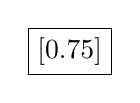
\begin{tikzpicture}
    \node[draw] {\usescalebox[0.75]\compFourBox};
\end{tikzpicture}
\caption{Expression tree of \figref{fig:PNBExprTreeConverted} after performing
all compositions}
\label{fig:exprtreestep4}
\end{figure}
